%\documentclass[CJK]{beamer}
%\usetheme[left,width=5em]{Goettingen}
\usepackage{fontspec}
\usepackage{xeCJK}
\makeatletter
\newcommand{\newinfo}[1]{}
\makeatother

\usepackage{fontspec,xunicode,xltxtra,listings}
\usepackage{breqn}
\usepackage[caption=false,font=footnotesize]{subfig}
\usepackage{tikz}
\usepackage{colortbl}
\usetikzlibrary{shapes,arrows,shadows,mindmap,backgrounds, shapes.multipart}
\usepackage{pgf-pie}
\graphicspath{{figures/}}
\DeclareGraphicsExtensions{.pdf,.png,.jpg}

\setbeamercovered{transparent}
\setbeamertemplate{items}[circle]
\setbeamertemplate{navigation symbols}{}

\renewcommand{\figurename}{Figure}


\newtheorem{definationfc}{Define}

\usepackage[overlap,CJK]{ruby}
\usepackage{multicol}
\usepackage[backend=bibtex]{biblatex}
\addbibresource{crossgap}
\usepackage{multirow,tabularx}

\newcommand{\backupbegin}{
   \newcounter{framenumberappendix}
   \setcounter{framenumberappendix}{\value{framenumber}}
}
\newcommand{\backupend}{
   \addtocounter{framenumberappendix}{-\value{framenumber}}
   \addtocounter{framenumber}{\value{framenumberappendix}}
}

\newcommand{\fcshadow}[1]{%
\hspace{-0.3em}\tikz[baseline]\path[anchor=base]%
node[fill opacity=0.1] at (0.05em,-0.05em) {#1}%
node[fill opacity=0.1] at (0.03em,-0.05em) {#1}%
node[fill opacity=0.1] at (0.05em,-0.03em) {#1}%
node[fill opacity=0.1] at (0.05em,-0.07em) {#1}%
node[fill opacity=0.1] at (0.07em,-0.05em) {#1}%
node at (0pt,0pt) {#1};\hspace{-0.4em}}%

\newcommand\bh{%
\tikz[remember picture, overlay]%
\coordinate(begin highlight){};%
}

\newcommand\eh{%
\tikz[remember picture, overlay]%
\coordinate (end highlight){};%
\tikz[remember picture, overlay,baseline=-0.65ex]%
\draw[red!50!black,line width=8pt,opacity=0.2] (begin highlight) -- (end highlight);%
}

\makeatletter
\newenvironment<>{btHighlight}[1][]
{\begin{onlyenv}#2\begingroup\tikzset{bt@Highlight@par/.style={#1}}\begin{lrbox}{\@tempboxa}}
{\end{lrbox}\bt@HL@box[bt@Highlight@par]{\@tempboxa}\endgroup\end{onlyenv}}

\newcommand<>\btHL[1][]{%
  \only#2{\begin{btHighlight}[#1]\bgroup\aftergroup\bt@HL@endenv}%
}
\def\bt@HL@endenv{%
  \end{btHighlight}%
  \egroup
}
\newcommand{\bt@HL@box}[2][]{%
  \tikz[#1]{%
    \pgfpathrectangle{\pgfpoint{1pt}{0pt}}{\pgfpoint{\wd #2}{\ht #2}}%
    \pgfusepath{use as bounding box}%
    \node[anchor=base west, fill=orange!30,outer sep=0pt,inner xsep=1pt, inner ysep=0pt, rounded corners=3pt, minimum height=\ht\strutbox+1pt,#1]{\raisebox{1pt}{\strut}\strut\usebox{#2}};
  }%
}
\makeatother

\setCJKsansfont[Mapping=tex-text]{Meiryo UI} %[Mapping=tex-text]
%\setCJKmonofont{Courier New}
\setCJKmonofont{Adobe Fangsong Std}
%\usefonttheme{structureitalicserif}
\usefonttheme{structurebold}
%\setmainfont[Mapping=tex-text]{Droid Serif}
%\setsansfont[Mapping=tex-text]{Droid Sans} %[Mapping=tex-text]
\setmonofont{Droid Sans Mono}
%\setmonofont{Lucida Sans Typewriter}

%\setbeamerfont{frametitle}{family=\fontspec{Apple Garamond}}
%\setbeamerfont{block title}{family=\fontspec{Apple Garamond}}

\def\beamer@linkspace#1{%
  \begin{pgfpicture}{0pt}{-1.5pt}{#1}{5.5pt}
    \pgfsetfillopacity{0}
    \pgftext[x=0pt,y=-1.5pt]{.}
    \pgftext[x=#1,y=5.5pt]{.}
  \end{pgfpicture}}


\renewcommand{\rubysep}{0.2ex}
\renewcommand{\rubysize}{0.6}

\lstset{tabsize=4, %
  language=Java,
  escapechar=`,
  frame=shadowbox, commentstyle=\color{green!20!black},
  rulesepcolor=\color{red!20!green!20!blue!20},
  keywordstyle=\color{blue!90}\bfseries,
  showstringspaces=false,
  stringstyle=\ttfamily,
  keepspaces=true, %
  breakindent=22pt, %
  numbers=left,%
  stepnumber=1,%
  numberstyle=\scriptsize, %
  basicstyle=\scriptsize\ttfamily, %
  showspaces=false, %
  flexiblecolumns=true, %
  breaklines=true, %
  breakautoindent=true,%
  breakindent=4em, %
  aboveskip=0.5em, %
  fontadjust,
  captionpos=t,
  framextopmargin=2pt,framexbottommargin=2pt,abovecaptionskip=-3pt,belowcaptionskip=3pt,
  xleftmargin=1.5em,xrightmargin=0.5em, %
  texcl=true,
  extendedchars=false,columns=flexible,mathescape=true,
  numbersep=0.5em,
}

\lstdefinestyle{sharpc}{language=[Sharp]C}
\newcommand{\upcite}[1]{\textsuperscript{\citep{#1}}}
%%%%%%%%%%%%%%%%%%%%%%%%%%%%%%%%%%%%%%%%%%%%%%%%%%%%%%%%%%%%%%%%%%%%%%%%


\title[Cross Gap from Imperative to Functional Refactoring]{Crossing the Gap from Imperative to Functional Programming through Refactoring}

\subtitle{MD輪講}

\author[大阪大学大学院CS専攻\quad{}楊 嘉晨]{博士後期課程2年\quad{}楊 嘉晨}
\institute[楠本研]{大阪大学大学院 コンピュータサイエンス専攻 楠本研究室}
\date{2014年5月29日(木)}

\mode<article>{\providecommand{\imageheight}{0.2\textheight}}
\mode<presentation>{\providecommand{\imageheight}{0.4\textheight}}


%%%%%%%%%%%%%%%%%%%%%%%%%%%%%%%%%%%%%%%%%%%%%%%%%%%%%%%%%%%%%%%%%%%%%%%%
\begin{document}

\mode<presentation>{

\providecommand{\newblock}{\\}
\providecommand{\toprule}{\hline}
\providecommand{\midrule}{\hline}
\providecommand{\bottomrule}{\hline}
\providecommand{\itemtitle}[1]{\item \alert{#1} \quad{} }
}

\mode<article>{
\renewenvironment{columns}{\begin{multicols}{2}}{\end{multicols}\\}
\renewenvironment{column}[1]{}{}
}

%\XeTeXlinebreaklocale "jp"
%\XeTeXlinebreakskip = 0pt plus 1pt
\frame{\titlepage}
\mode<article>{\maketitle}

\begin{frame}<trans|beamer|handout|notes>

\tableofcontents[sectionstyle=show/show,subsectionstyle=hide,subsubsectionstyle=hide]
\end{frame}


\AtBeginSubsection[]{
\begin{frame}<trans|beamer|handout|notes>%{Agenda: \insertsection}
\begin{center}
%\Huge\insertsection
\tableofcontents[sectionstyle=show/shaded,subsectionstyle=show/shaded/hide]
\end{center}
\end{frame}
}
%%%%%%%%%%%%%%%%%%%%%%%%%%%%%%%%%%%%%%%%%%%%%%%%%%%%%%%%%%%%%%%%%%%%%%%%
\section{背景と動機の例}
\subsection{出典(Publication)}
\begin{frame}{出典}{Publication}

\emph{タイトル}: \fcshadow{手続き型}と\fcshadow{関数型}プログラミングの隙間を越え

ESEC/FSE 2013
\begin{itemize}
\item 10 ページ + 参考文献
\item {\small Joint Meeting of
the European Software Engineering Conference and
the ACM SIGSOFT Symposium
on the Foundations of Software Engineering}
\end{itemize}
Alex Gyori (米Illinois大), Lyle Franklin\footfullcite{franklin2013lambdaficator} (米Ball州立大),\\
{\small Danny Dig (米Oregon州立大), and Jan Lahoda (Oracle)}
\end{frame}
%%%%%%%%%%%%%%%%%%%%%%%%%%%%%%%%%%%%%%%%%%%%%%%%%%%%%%%%%%%%%%%%%%%%%%%
\subsection{背景:ラムダ式(Lambda Expressions)}
\begin{frame}[fragile]{Java 8におけるラムダ式}{Lambda Expression in Java 8}
ラムダ式(匿名関数ともいう)は名前がない関数、Java 8から支援
\begin{lstlisting}[moredelim={**[is][{\btHL}]{*1}{*}}]
blocks.stream().filter(*1b -> b.getColor() == BLUE*)
\end{lstlisting}
これまでJavaに匿名内部クラス(Anonymous Inner Class, AIC)で書かれていた
単純な処理をより簡単に書ける.
\pause
上記と同じ処理を従来の書き方:
\begin{columns}
\begin{column}{0.5\textwidth}
\begin{block}{拡張for文}
\begin{lstlisting}
List<Block> result = new ArrayList<>();
for(Block b:blocks){
  if(b.getColor() == BLUE){
    result.add(b);
  }
}
\end{lstlisting}
\end{block}
\end{column}
\begin{column}{0.47\textwidth}
\begin{block}{AICとstreamを使う}
\begin{lstlisting}
blocks.stream().filter(
  new Predicate<Block>(){
    @Override boolean test(Block b){
      return b.getColor() == BLUE;
    }
})
\end{lstlisting}
\end{block}
\end{column}
\end{columns}
\end{frame}
%%%%%%%%%%%%%%%%%%%%%%%%%%%%%%%%%%%%%%%%%%%%%%%%%%%%%%%%%%%%%%%%%%%%%%%%

\begin{frame}[fragile]{関数型に変換による並列化}
\begin{columns}
\begin{column}{0.57\textwidth}
ラムダ式の導入によって書き方が簡単にするだけでなく、並列化も簡単になれる
\begin{block}{逐次処理}
\begin{lstlisting}
for(ElementRule r:properties.getRules()){
  r.resetHierarchy();
}
\end{lstlisting}
\end{block}
\begin{block}{新式の並列化}
\begin{lstlisting}[morekeywords={parallelStream, forEach},moredelim={**[is][{\btHL}]{*1}{*}}]
properties.getRules().parallelStream().
  forEach(*1(ElementRule r) ->*
    *1r.resetHierarchy()*);
\end{lstlisting}
\end{block}
\end{column}
\begin{column}{0.4\textwidth}
\begin{block}{旧式の並列化}
\begin{lstlisting}[basicstyle=\tiny]
int n = 4; // amount of parallelism
Thread[] threads = new Thread[n];
final List<ElementRule> rules=properties.getRules();
int size = rules.size();
for (int i=0; i<n; i++){
  final int from = i * size / n;
  final int to = (i + 1) * size / n;
  thread[i] = new Thread(new Runnable(){
    @Override public void run(){
      for (int j = from ; j < to ; j++){
        rules.get(j).resetHierarchy();
  }}});
  threads[i].start();
}
for(int i=0; i<n; ++i){
  try{
    threads[i].join();
  } catch (InterruptedException ex) {
    // print error message
  }
}
\end{lstlisting}
\end{block}
\end{column}
\end{columns}
\end{frame}
%%%%%%%%%%%%%%%%%%%%%%%%%%%%%%%%%%%%%%%%%%%%%%%%%%%%%%%%%%%%%%%%%%%%%%%%
\subsection{この研究の貢献(Contributions)}
\begin{frame}{この研究の貢献}{Contributions}
  2つのリファクタリング手法を提案いたします
  \begin{description}
    \item[AnonymousToLambda] AICからラムダ式に変換
    \item[ForLoopToFunctional] 拡張for文からラムダ式を用いて関数型に変換
  \end{description}
  NetBeansの機能として実装し、次のバージョンに提供

  9個、総行数百万行越え、性質が違うプロジェクトで評価
  \begin{itemize}
    \item 汎用性が高い。 ATLは55\%,FLTFは46\%適用可能
    \item 精度が高い。 正解集合と比べてATLは100\%, FLTFは90\%以上
  \end{itemize}

  ツールと実験データは公開
  \footnote{\url{http://refactoring.info/tools/LambdaFicator}}
  \footnote{\url{http://www.youtube.com/watch?v=EIyAflgHVpU}}
\end{frame}
%%%%%%%%%%%%%%%%%%%%%%%%%%%%%%%%%%%%%%%%%%%%%%%%%%%%%%%%%%%%%%%%%%%%%%%%
\subsection{AnonymousToLambdaの例}
\begin{frame}[fragile]{AICからラムダ式に変換\footfullcite{lambda2011state}}
\begin{block}{匿名内部クラス(AIC)}
\begin{lstlisting}[moredelim={**[is][{\btHL<2>}]{*2}{*}}]
button.addActionListener(*2new ActionListener(){*
  *2public void actionPerformed*(ActionEvent e) {
    ui.dazzle(e.getModifiers());
  *2}*
});
\end{lstlisting}
\end{block}
\begin{block}{相当するラムダ式}
\begin{lstlisting}[moredelim={**[is][{\btHL<2>}]{*2}{*}}]
button.addActionListener((ActionEvent e) *2->* {
    ui.dazzle(e.getModifiers());
});
\end{lstlisting}
\end{block}
\end{frame}
%%%%%%%%%%%%%%%%%%%%%%%%%%%%%%%%%%%%%%%%%%%%%%%%%%%%%%%%%%%%%%%%%%%%%%%%
\begin{frame}[fragile]{AICからラムダ式に変換する場合に特殊の例}
\begin{columns}
\begin{column}{0.6\textwidth}
\begin{block}{匿名内部クラス(AIC)}
\begin{lstlisting}[moredelim={**[is][{\btHL<3>}]{*3}{*}}]
String sep = doAction(new PrivilegedAction()*3{*
  public String run(){
    *3return* System.getProperty("file.separator");
  }
*3}*);
\end{lstlisting}
\end{block}
\begin{block}{ラムダ式に型変換が必要}
\begin{lstlisting}[moredelim={**[is][{\btHL<2>}]{*1}{*}},moredelim={**[is][{\btHL<3>}]{*3}{*}}]
String sep = doAction(*1(PrivilegedAction)*() *1->*
  System.getProperty("file.separator")
);
\end{lstlisting}
\end{block}
\end{column}
\begin{column}{0.4\textwidth}
\begin{uncoverenv}<2>
呼びだされた\texttt{doAction}の定義は:
\begin{lstlisting}
doAction(PrivilegedAction)
doAction(ExceptionAction)
\end{lstlisting}
変換するだけでは曖昧な二択問題が生じる
\end{uncoverenv}

\uncover<3->{
\texttt{return}文だけのラムダ式では表現式だけで十分
}
\end{column}
\end{columns}
\end{frame}

%%%%%%%%%%%%%%%%%%%%%%%%%%%%%%%%%%%%%%%%%%%%%%%%%%%%%%%%%%%%%%%%%%%%%%%%
\subsection{ForLoopToFunctionalの例}
\begin{frame}[fragile]{ForLoopToFunctionalの例1}

\begin{lstlisting}[moredelim={**[is][{\btHL<2>}]{*2}{*}},
  moredelim={**[is][{\btHL<3>}]{*3}{*}},
  moredelim={**[is][{\btHL<4>}]{*4}{*}}]
class GrammarEngineImpl implements GrammarEngine{
  boolean isEngineExisting(String grammarName){
    for(GrammarEngine e : importedEngines){
      *2if(e.getGrammarName() == null) continue;*
      *3if(e.getGrammarName().equals(grammarName))*
        *3return true;*
    }
    return false;
  }
}
\end{lstlisting}
\begin{lstlisting}[morekeywords={filter,stream,anyMatch,map,reduce,forEach},
  moredelim={**[is][{\btHL<2>}]{*2}{*}},
  moredelim={**[is][{\btHL<3>}]{*3}{*}},
  moredelim={**[is][{\btHL<4>}]{*4}{*}}]
class GrammarEngineImpl implements GrammarEngine{
  boolean isEngineExisting(String grammarName){
    return importedEngines.stream()
      *2.filter*(*4e ->* e.getGrammarName() != null)
      *3.anyMatch*(*4e ->* e.getGrammarName().equals(grammarName));
  }
}
\end{lstlisting}
\end{frame}
\begin{frame}[fragile]{ForLoopToFunctionalの例2}

\begin{lstlisting}[moredelim={**[is][{\btHL<2>}]{*2}{*}},
  moredelim={**[is][{\btHL<3>}]{*3}{*}},
  moredelim={**[is][{\btHL<4>}]{*4}{*}}]
class EditorGutterColumnManager{
  int getNumberOfErrors(){
    int count = 0;
    for(ElementRule rule : getRules()){
      *2if(rule.hasErrors()){*
        *4count +=* *3rule.getErrors().size();*
      }
    }
    return count;
  }
}
\end{lstlisting}
\begin{lstlisting}[morekeywords={filter,stream,anyMatch,map,reduce,forEach},
  moredelim={**[is][{\btHL<2>}]{*2}{*}},
  moredelim={**[is][{\btHL<3>}]{*3}{*}},
  moredelim={**[is][{\btHL<4>}]{*4}{*}},
  moredelim={**[is][{\btHL<5>}]{*5}{*}}]
class EditorGutterColumnManager{
  int getNumberOfErrors(){
    return getRules().stream()
      .*2filter(rule -> rule.hasErrors())*
      .*3map(rule -> rule.getErrors().size())*
      .*4reduce*(0, *5Interger::plus*);           // method reference in Java 8
  }
}
\end{lstlisting}
\end{frame}
\begin{frame}[fragile]{ForLoopToFunctionalの例3}

\begin{lstlisting}[moredelim={**[is][{\btHL<2>}]{*2}{*}},
moredelim={**[is][{\btHL<3>}]{*3}{*}}]
List<String> findReloadedContextMemoryLeaks()){
  List<String> result = new ArrayList<String>();
  for(Map.Entry<ClassLoader, String> entry: childClassLoaders.entrySet())
    *2if(isValid(entry)){*
      *3ClassLoader cl = entry.getKey();*
      *3if (!((WebappClassLoader)cl).isStart())*
        *3result.add(entry.getValue());*
    }
  ...
}
\end{lstlisting}
\begin{lstlisting}[morekeywords={filter,stream,anyMatch,map,reduce,forEach},
  moredelim={**[is][{\btHL<2>}]{*2}{*}},
  moredelim={**[is][{\btHL<3>}]{*3}{*}}]
List<String> findReloadedContextMemoryLeaks()){
  List<String> result = new ArrayList<String>();
  childClassLoaders.entrySet().stream()
    .*2filter(entry -> isValid(entry))*
    .*3forEach(entry -> {*
      *3ClassLoader cl = entry.getKey();*
      *3if (!((WebappClassLoader)cl).isStart())*
        *3result.add(entry.getValue());}*);
  ...
}
\end{lstlisting}
\end{frame}
%%%%%%%%%%%%%%%%%%%%%%%%%%%%%%%%%%%%%%%%%%%%%%%%%%%%%%%%%%%%%%%%%%%%%%%%
\section{AnonymousToLambdaのリファクタリング}
\subsection{ツールの使い方 Workflow}
\begin{frame}{ツールの使い方: Quick Hint Mode}
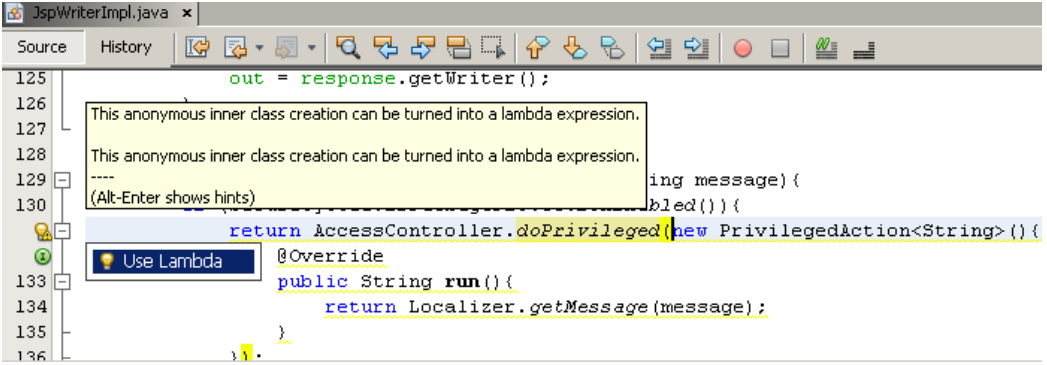
\includegraphics[width=\textwidth]{quickhint}
\end{frame}
%%%%%%%%%%%%%%%%%%%%%%%%%%%%%%%%%%%%%%%%%%%%%%%%%%%%%%%%%%%%%%%%%%%%%%%%
\begin{frame}{ツールの使い方: Batch Mode}
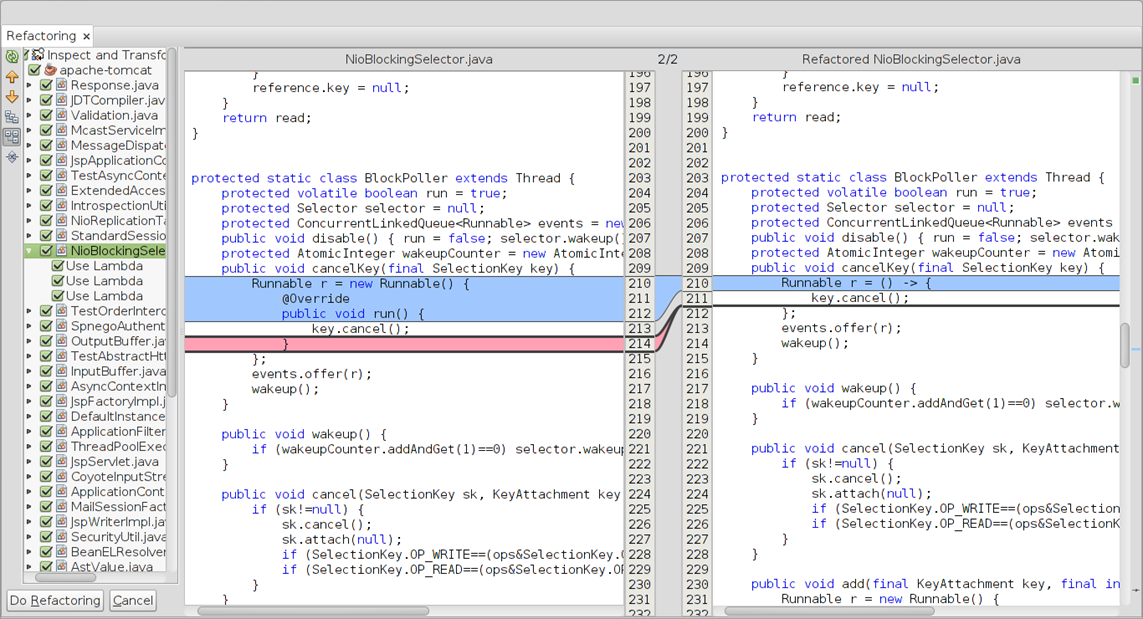
\includegraphics[width=\textwidth, height=0.9\textheight, keepaspectratio]{batch}
\end{frame}
%%%%%%%%%%%%%%%%%%%%%%%%%%%%%%%%%%%%%%%%%%%%%%%%%%%%%%%%%%%%%%%%%%%%%%%%
\subsection{Javaの型システムにおけるラムダの実装}
\begin{frame}[fragile]{Javaの型システムにおけるラムダの実装}{Lambda Expression Implementation}
Python, C\# (3.0以降) 等にラムダ式の型は特殊な\fcshadow{関数}型になる
\begin{columns}
\begin{column}{0.5\textwidth}
\begin{block}{Pythonのラムダ式}
\begin{lstlisting}[language=Python]
>>> type(lambda x: x==5)
<class 'function'>
\end{lstlisting}
\end{block}
\end{column}
\begin{column}{0.5\textwidth}
\begin{block}{C\#のラムダ式}
\begin{lstlisting}[style=sharpc]
Func<int, bool> myFunc = x => x == 5;
\end{lstlisting}
\end{block}
\end{column}
\end{columns}
\begin{uncoverenv}<2->
Java 8に相当する型は存在しないが、関数インターフェイスを使う
\begin{columns}
\begin{column}{0.5\textwidth}
\begin{block}{Java 8のラムダ式}
\begin{lstlisting}
BinaryOperator sum = (x,y) -> x + y;
\end{lstlisting}
\end{block}
\end{column}
\begin{column}{0.5\textwidth}
\begin{block}{関数インターフェイス}
\begin{lstlisting}
interface BinaryOperator<T>{
  T op(T a, T b);
}
\end{lstlisting}
\end{block}
\end{column}
\end{columns}
\end{uncoverenv}
\end{frame}
%%%%%%%%%%%%%%%%%%%%%%%%%%%%%%%%%%%%%%%%%%%%%%%%%%%%%%%%%%%%%%%%%%%%%%%%
\subsection{事前条件(Preconditions)}
\begin{frame}{事前条件}{Preconditions}
AICをラムダ式に変換できるのは、これらの事前条件に守れるものである
\begin{itemize}
  \item[P1] AICはインターフェイスを実装する\footfullcite{java8lambda}\\
            クラスを実装するAICは変換できない
  \item[P2] AICにフィルドがない, メソットが一つだけ\footfullcite{java8functionalinterfaces}\\
            複数以上のメソットで変換できない
  \item[P3] AICに\texttt{this}と\texttt{super}は使っていない\\
            AICの\texttt{this}はAIC自身を指すが, ラムダ式に相当物がない
  \item[P4] AICに定義したメソットは再帰的ではない \uncover<2>{(Y-combinatorできる?)}
\end{itemize}
\end{frame}
%%%%%%%%%%%%%%%%%%%%%%%%%%%%%%%%%%%%%%%%%%%%%%%%%%%%%%%%%%%%%%%%%%%%%%%%
\subsection{特殊の処理(Special Cases)}
\begin{frame}{特殊の処理}{Special Cases}
AICからラムダ式に変換する自体は簡単

要らない部分を削除したらできる

\begin{itemize}
  \item[S1] \texttt{return}文のみの場合に関数のブロックを省略
  \item[S2] AICの型と代入されたところの型が違った場合に型変換を挿入
  \item[S3] AICを使うメソットがoverloadされた場合にも型変換を挿入
  \item[S4] AIC内部に定義されたローカル変数は外部のローカル変数と名前と被った場合に, 一意な名前をつける
\end{itemize}

\end{frame}
%%%%%%%%%%%%%%%%%%%%%%%%%%%%%%%%%%%%%%%%%%%%%%%%%%%%%%%%%%%%%%%%%%%%%%%%
\section{ForLoopToFunctionalのリファクタリング}
\subsection{対象となるJava 8の新しい操作}
\begin{frame}[fragile]{対象となるJava 8の新しい操作}{New Operations in Java 8}
目的:拡張for文で書かれた処理を、次の操作の連鎖(chain)に変換
\begin{lstlisting}[keywords={map,filter,reduce,forEach,anyMatch,noneMatch}]
package java.util.stream;
interface Steam<T> ... {
  Stream<R> map(Function<? super T, ? extends R> mapper); //lazy
  Stream<T> filter(Predicate<? super T> predicate);       //lazy
  T reduce(T identity, BinaryOperator<T> reducer);        //eager
  void forEach(Consumer<? super T> consumer);             //eager
  boolean anyMatch(Predicate<? super T> predicate);       //eager, short-circuiting
  boolean noneMatch(Prediate<? super T> predicate);       //eager, short-circuiting
  ...
}
\end{lstlisting}
ただし、拡張for文の意味がeagerである以上、連鎖操作の最後はeagerであるべき
\end{frame}

%%%%%%%%%%%%%%%%%%%%%%%%%%%%%%%%%%%%%%%%%%%%%%%%%%%%%%%%%%%%%%%%%%%%%%%%
\subsection{事前条件(Preconditions)}
\begin{frame}{事前条件}{Preconditions}
拡張for文で書かれた処理の内、ラムダ式に含まれないものがある
\begin{itemize}
  \item[P1] 配列ではなく, Collectionのオブジェクトを対象とする\\
            {\small Collectionからstreamを得られるから}
  \item[P2] チェック例外を外に投げない\\
            {\small ラムダ式に\texttt{throws}文がないから}
  \item[P3] 非finalのローカル変数を一つ以上参照しない\\
            {\small 事実上ローカル変数の前にfinalをつけるなら問題なし\\
            一つだけの場合に\texttt{reduce}に変換するヒューリスティック法がある}
  \item[P4-6] \texttt{break, return, continue} 文が存在しない \\
            {\small return boolean文が一つの場合に\texttt{anyMatch/noneMatch}に変換するヒューリスティック法がある(後述) \\
            ラベル無しcontinue文の場合に事前にリファクタリングによって削る}
\end{itemize}
\end{frame}
%%%%%%%%%%%%%%%%%%%%%%%%%%%%%%%%%%%%%%%%%%%%%%%%%%%%%%%%%%%%%%%%%%%%%%%%
\subsection{変換方法(Algorithm)}
\begin{frame}{変換方法}{Algorithm}
  入力:拡張for文 \quad 出力:連鎖された一連の操作 \\
  難しい点:for文内に定義されたローカル変数の作用範囲が変わる
  \begin{description}
    \item[Step 1] 拡張for文のブロックを文単位で潜在操作(Prospective Operation, OP)に分割 \\
              {\small \texttt{else}がない\texttt{if}文 $\rightarrow$ \texttt{filter}\\
              他の文 $\rightarrow$ \texttt{map} \\
              最後の文 $\rightarrow$ \texttt{eager}}
    \item[Step 2] 分割した操作に、変数を使わられた情報を注釈
    \item[Step 3] 変数依存によって、連鎖できない操作をマージ
    \item[Step 4] 操作を連鎖させ
  \end{description}
\end{frame}
%%%%%%%%%%%%%%%%%%%%%%%%%%%%%%%%%%%%%%%%%%%%%%%%%%%%%%%%%%%%%%%%%%%%%%%%
\begin{frame}{Step 2 変数を使わられた情報を注釈}
拡張for文にある各潜在操作$PO$に対し
\begin{itemize}
  \item[$F$] すべてのアクセスできるフィルド変数
  \item[$L_{PO}$] $PO$に定義したローカル変数
  \item[$L_{Meth}$] 現在のメソッドに全てのローカル変数
  \item[$L_{Loop}$] 拡張for文に定義した全てのローカル変数
  \item[$U_{PO}$] $PO$に使われた変数
\end{itemize}
したがって、使える変数は:$AV_{PO} = F \cup L_{PO} \cup \{ L_{Meth} \backslash L_{Loop} \}$ \\
必要される変数は:$NV_{PO} = U_{PO} \backslash AV_{PO}$
\end{frame}

%%%%%%%%%%%%%%%%%%%%%%%%%%%%%%%%%%%%%%%%%%%%%%%%%%%%%%%%%%%%%%%%%%%%%%%%
\begin{frame}{Step 3 連鎖できない操作をマージ}
2つの潜在操作$O$と$O'$に関して、連鎖させるか ($O.O'$) をチェックする

即ち,後ろの操作$O'$に必要な変数を前の操作$O$から得られるかのチェック
\begin{displaymath}
  (O.O') \quad \textit{iff} \quad |NV_{O'}|=1 \quad \textit{and} \quad NV_{O'} \subseteq (AV_O \cup NV_O)
\end{displaymath}
連鎖できない場合に、 $O$と$O'$の2つの操作をマージして$O''$になり
\[AV_{O''} = AV_O \cup AV_{O'} \quad NV_{O''}=\{NV_O \cup NV_{O'}\} \backslash AV_{O''}\]
\end{frame}
%%%%%%%%%%%%%%%%%%%%%%%%%%%%%%%%%%%%%%%%%%%%%%%%%%%%%%%%%%%%%%%%%%%%%%%%
\begin{frame}{Step 4 操作を連鎖させ}
最後の操作はeagerであるべきから、次のヒューリスティック法を使う
\begin{description}
  \item[reduce] 一つだけ非finalローカル変数に対し, このいずれの計算をしている:
                \texttt{+=, -=, *=, /=, \%=, |=, \&=, <<=, >>=, ++, --}
  \item[anyMatch] \texttt{return true}
  \item[noneMatch] \texttt{return false}
  \item[forEach] 非finalローカル変数を使ってない, かつ\texttt{return}文がない
\end{description}
最後の操作を決められたら、逆順で前の操作を一つずつ繋ぎあげる。
\end{frame}

%%%%%%%%%%%%%%%%%%%%%%%%%%%%%%%%%%%%%%%%%%%%%%%%%%%%%%%%%%%%%%%%%%%%%%%%
\begin{frame}[fragile]{動機の例の例3を用いて説明}

\begin{onlyenv}<1,2>
\begin{lstlisting}
List<String> result = new ArrayList<>();
for(Map.Entry<ClassLoader, String> entry: childClassLoaders.entrySet())
  if(isValid(entry)){
    ClassLoader cl = entry.getKey();
    if (!((WebappClassLoader)cl).isStart())
      result.add(entry.getValue());
  }
\end{lstlisting}
\uncover<2>{
事前条件の確認
\begin{itemize}
  \item[P1] SetはCollection
  \item[P2] 例外を投げ出していない
  \item[P3] for文外のローカル変数は result, for文内に代入していない, 実質上finalである
  \item[P4-6] \texttt{return, break, continue}文がない
\end{itemize}
}
\end{onlyenv}
\begin{onlyenv}<3>
Step 1, 拡張for文のブロックを文単位でOPに分割
\begin{lstlisting}
List<String> result = new ArrayList<>();
for(Map.Entry<ClassLoader, String> entry: childClassLoaders.entrySet())
\end{lstlisting}
\begin{lstlisting}
  if(isValid(entry)){                        // PO1: Filter
\end{lstlisting}
\begin{lstlisting}
    ClassLoader cl = entry.getKey();         // PO2: Map
\end{lstlisting}
\begin{lstlisting}
    if (!((WebappClassLoader)cl).isStart())  // PO3: Filter
\end{lstlisting}
\begin{lstlisting}
      result.add(entry.getValue());          // PO4: Eager
\end{lstlisting}
\begin{lstlisting}
  }
\end{lstlisting}
\end{onlyenv}
\begin{onlyenv}<4>
Step 2, 変数を使わられた情報を注釈
\begin{lstlisting}
List<String> result = new ArrayList<>();
for(Map.Entry<ClassLoader, String> entry: childClassLoaders.entrySet())
\end{lstlisting}
\begin{lstlisting}
  if(isValid(entry)){                        // PO1: Filter, AV=\{\}, NV=\{entry\}
\end{lstlisting}
\begin{lstlisting}
    ClassLoader cl = entry.getKey();         // PO2: Map, AV=\{cl\}, NV=\{entry\}
\end{lstlisting}
\begin{lstlisting}
    if (!((WebappClassLoader)cl).isStart())  // PO3: Filter, AV=\{\}, NV=\{cl\}
\end{lstlisting}
\begin{lstlisting}
      result.add(entry.getValue());          // PO4: Eager, AV=\{result\}, NV=\{entry\}
\end{lstlisting}
\begin{lstlisting}
  }
\end{lstlisting}
\end{onlyenv}
\begin{onlyenv}<5>
Step 3, 共通変数がある操作をマージ\\
$NV_{O4} = \{\text{entry}\} \nsubseteq (AV_{O3} \cup NV_{O3}) = \{\text{cl}\}$ マージすべき
\begin{lstlisting}
List<String> result = new ArrayList<>();
for(Map.Entry<ClassLoader, String> entry: childClassLoaders.entrySet())
\end{lstlisting}
\begin{lstlisting}
  if(isValid(entry)){                        // PO1: Filter, AV=\{\}, NV=\{entry\}
\end{lstlisting}
\begin{lstlisting}
    ClassLoader cl = entry.getKey();         // PO2: Map, AV=\{cl\}, NV=\{entry\}
\end{lstlisting}
\begin{lstlisting}
    if (!((WebappClassLoader)cl).isStart())  // PO3: Filter, AV=\{\}, NV=\{cl\}
\end{lstlisting}
\begin{lstlisting}
      result.add(entry.getValue());          // PO4: Eager, AV=\{result\}, NV=\{entry\}
\end{lstlisting}
\begin{lstlisting}
  }
\end{lstlisting}
\end{onlyenv}
\begin{onlyenv}<6>
Step 3, 共通変数がある操作をマージ\\
$| NV_{O3} = \{\text{entry, cl}\}| > 1$ マージすべき
\begin{lstlisting}
List<String> result = new ArrayList<>();
for(Map.Entry<ClassLoader, String> entry: childClassLoaders.entrySet())
\end{lstlisting}
\begin{lstlisting}
  if(isValid(entry)){                        // PO1: Filter, AV=\{\}, NV=\{entry\}
\end{lstlisting}
\begin{lstlisting}
    ClassLoader cl = entry.getKey();         // PO2: Map, AV=\{cl\}, NV=\{entry\}
\end{lstlisting}
\begin{lstlisting}
    if (!((WebappClassLoader)cl).isStart())
      result.add(entry.getValue());  // PO3: Eager, AV=\{result\}, NV=\{cl, entry\}
\end{lstlisting}
\begin{lstlisting}
  }
\end{lstlisting}
\end{onlyenv}
\begin{onlyenv}<7>
Step 3, 共通変数がある操作をマージ\\
連鎖できる
\begin{lstlisting}
List<String> result = new ArrayList<>();
for(Map.Entry<ClassLoader, String> entry: childClassLoaders.entrySet())
\end{lstlisting}
\begin{lstlisting}
  if(isValid(entry)){                        // PO1: Filter, AV=\{\}, NV=\{entry\}
\end{lstlisting}
\begin{lstlisting}
    ClassLoader cl = entry.getKey();   // PO2: Eager, AV=\{cl,result\}, NV=\{entry\}
    if (!((WebappClassLoader)cl).isStart())
      result.add(entry.getValue());
\end{lstlisting}
\begin{lstlisting}
  }
\end{lstlisting}
\end{onlyenv}
\begin{onlyenv}<8>
Step 4, 操作を連鎖させ
\begin{lstlisting}
List<String> result = new ArrayList<>();
for(Map.Entry<ClassLoader, String> entry: childClassLoaders.entrySet())
\end{lstlisting}
\begin{lstlisting}
  if(isValid(entry)){                        // PO1: Filter, AV=\{\}, NV=\{entry\}
\end{lstlisting}
\begin{lstlisting}
    ClassLoader cl = entry.getKey();  // PO2: forEach, AV=\{cl,result\}, NV=\{entry\}
    if (!((WebappClassLoader)cl).isStart())
      result.add(entry.getValue());
\end{lstlisting}
\begin{lstlisting}
  }
\end{lstlisting}
\end{onlyenv}
\begin{onlyenv}<9>
Step 4, 操作を連鎖させ
\begin{lstlisting}
List<String> result = new ArrayList<>();
childClassLoaders.entrySet().stream()
\end{lstlisting}
\begin{lstlisting}[morekeywords={map,filter,reduce,forEach,anyMatch,noneMatch}]
  .filter( entry -> isValid(entry))
\end{lstlisting}
\begin{lstlisting}[morekeywords={map,filter,reduce,forEach,anyMatch,noneMatch}]
  .forEach( entry -> {
    ClassLoader cl = entry.getKey();
    if (!((WebappClassLoader)cl).isStart())
      result.add(entry.getValue());
      })
\end{lstlisting}
\end{onlyenv}
\begin{onlyenv}<10>
Step 4, 操作を連鎖させ
\begin{lstlisting}[morekeywords={map,filter,reduce,forEach,anyMatch,noneMatch}]
List<String> result = new ArrayList<>();
childClassLoaders.entrySet().stream()
  .filter( entry -> isValid(entry))
  .forEach( entry -> {
    ClassLoader cl = entry.getKey();
    if (!((WebappClassLoader)cl).isStart())
      result.add(entry.getValue());
  });
\end{lstlisting}
\end{onlyenv}
\end{frame}
%%%%%%%%%%%%%%%%%%%%%%%%%%%%%%%%%%%%%%%%%%%%%%%%%%%%%%%%%%%%%%%%%%%%%%%%
\section{評価実験(Evaluation)}
\subsection{実験設定(Experimental Setup)}
\begin{frame}{Research Questions}
\begin{description}
\item[Q1. 汎用] リファクタリングはどのぐらい汎用できる?
\item[Q2. 価値] コードの品質を向上した?
\item[Q3. 効果] プログラマーの仕事をどのぐらいに楽にしたのか?
\item[Q4. 精度] batch modeで実行したらどのぐらいの精度がある?
\item[Q5. 安全] 安全に使える?
\end{description}
\end{frame}
%%%%%%%%%%%%%%%%%%%%%%%%%%%%%%%%%%%%%%%%%%%%%%%%%%%%%%%%%%%%%%%%%%%%%%%%
\begin{frame}{実験設定}{Experimental Setup}
\begin{columns}
\begin{column}{0.7\textwidth}
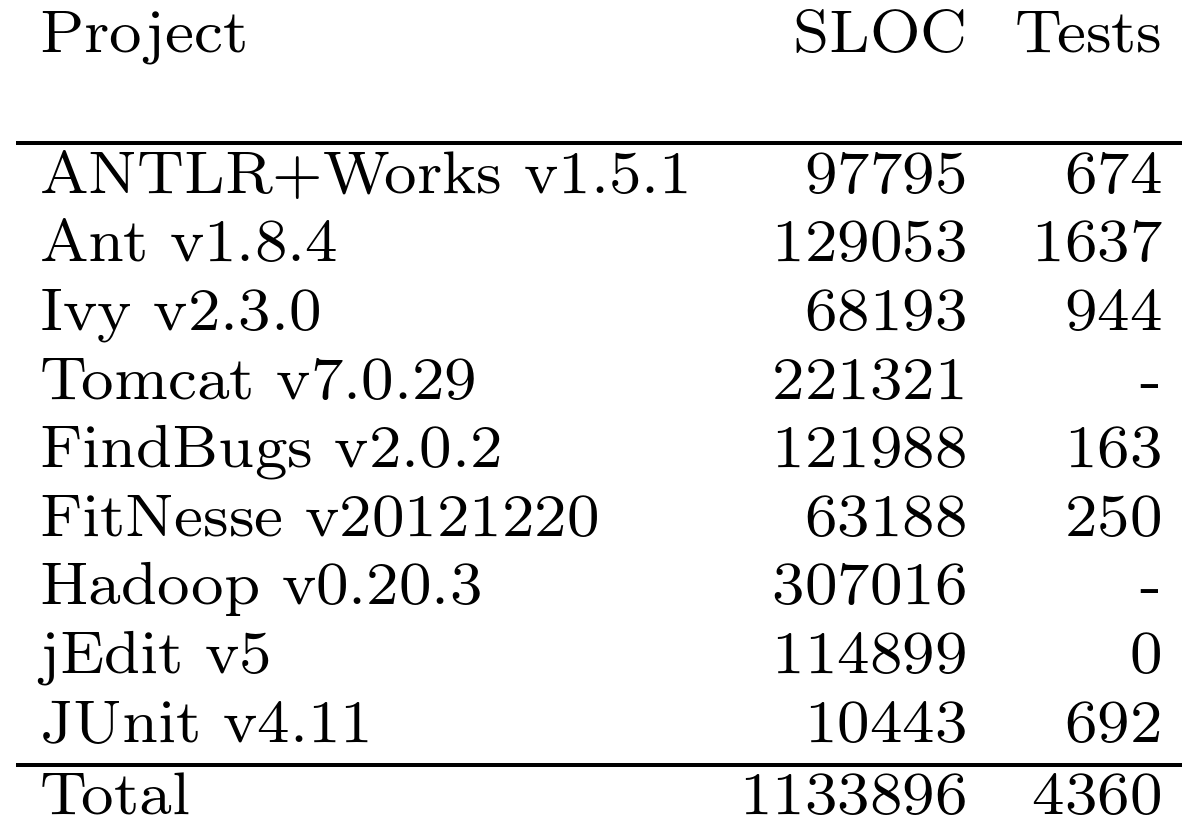
\includegraphics[width=\textwidth,height=.8\textheight,keepaspectratio]{target}
\end{column}
\begin{column}{0.3\textwidth}
  \pause 総行数は百万行越え

  \pause jEditにJUnitのテストケースがない

  \pause TomcatとHadoopは、Java 8でテストケースが実行不可能
\end{column}
\end{columns}
\end{frame}
%%%%%%%%%%%%%%%%%%%%%%%%%%%%%%%%%%%%%%%%%%%%%%%%%%%%%%%%%%%%%%%%%%%%%%%%
\begin{frame}{評価指標}{Evaluation Metrics}
batch mode でリファクタリングを適用
\begin{description}
  \item[Q1. 汎用] 適用された数と比率、事前条件や特殊処理の数
  \item[Q2. 価値] 行数とASTのノード数に減らされた数
  \item[Q3. 効果] 変更を加えたファイル数と行数、実行時間
\end{description}
全部対象のなかで10\%を選んで、もどのソースコードを専門家に任せて、手作業で
正解集合を作る
\begin{description}
  \item[Q4. 精度] ツールの出力と正解集合と比べてrecallとprecisionで評価
  \item[Q5. 安全] 配布されたJUnitを実行し、変換前後新たな障害が起こらず\\
                  手作業で10\%を確認し、コードの意味が変わらず
\end{description}
\end{frame}
%%%%%%%%%%%%%%%%%%%%%%%%%%%%%%%%%%%%%%%%%%%%%%%%%%%%%%%%%%%%%%%%%%%%%%%%
\subsection{AnonymousToLambdaの実験}
\begin{frame}{AnonymousToLambdaの汎用性}
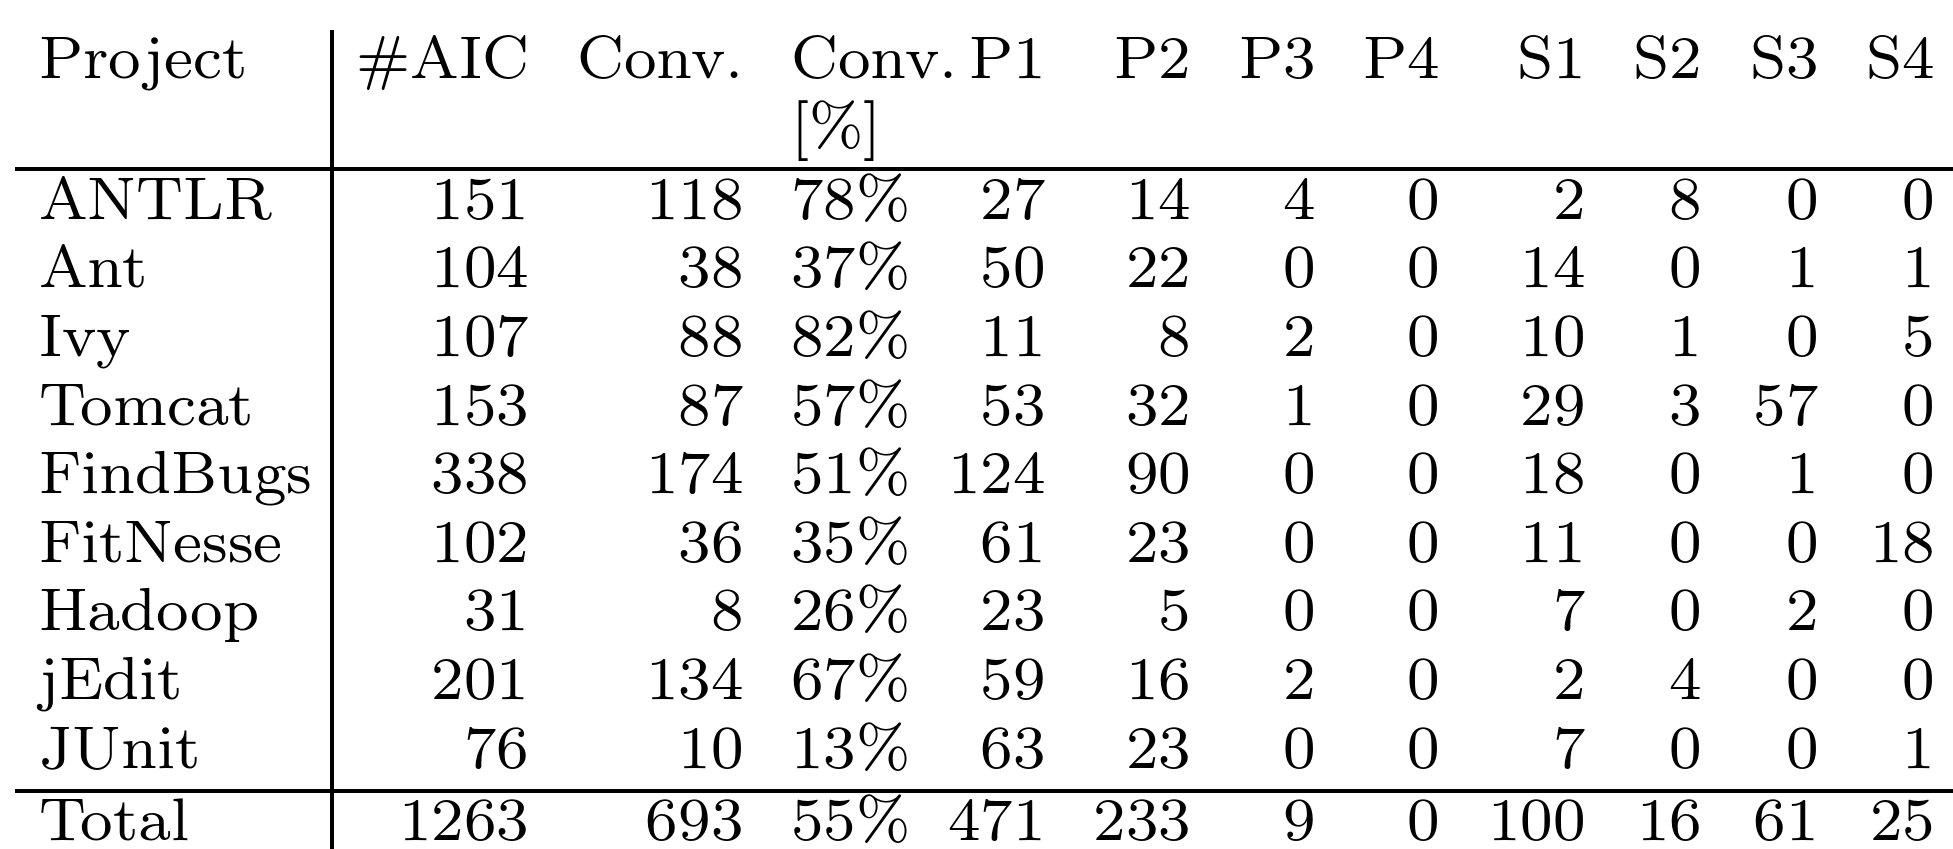
\includegraphics[width=\textwidth,height=.8\textheight,keepaspectratio]{aicapp}
\end{frame}

\begin{frame}{AnonymousToLambdaの価値、効果と精度}
\begin{columns}
  \begin{column}{0.7\textwidth}
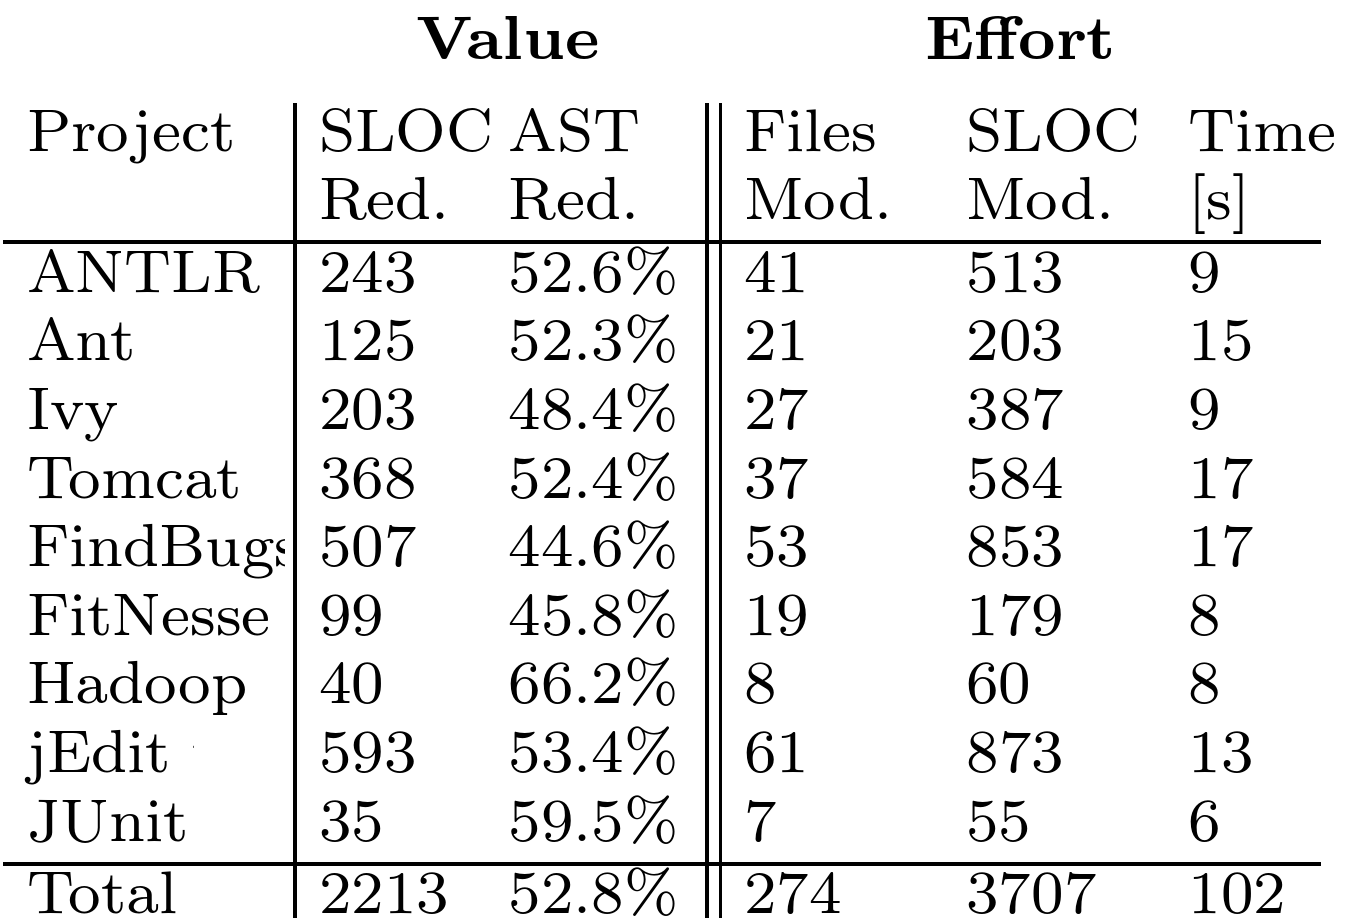
\includegraphics[width=\textwidth,height=.8\textheight,keepaspectratio]{aicvalue}
\end{column}
\begin{column}{0.3\textwidth}
  精度に関して\\
  recall = 100\%
  precision = 100\%
\end{column}
\end{columns}
\end{frame}
%%%%%%%%%%%%%%%%%%%%%%%%%%%%%%%%%%%%%%%%%%%%%%%%%%%%%%%%%%%%%%%%%%%%%%%%
\subsection{ForLoopToFunctionalの実験}
\begin{frame}{ForLoopToFunctionalの汎用性}
  \begin{columns}
    \begin{column}{0.8\textwidth}
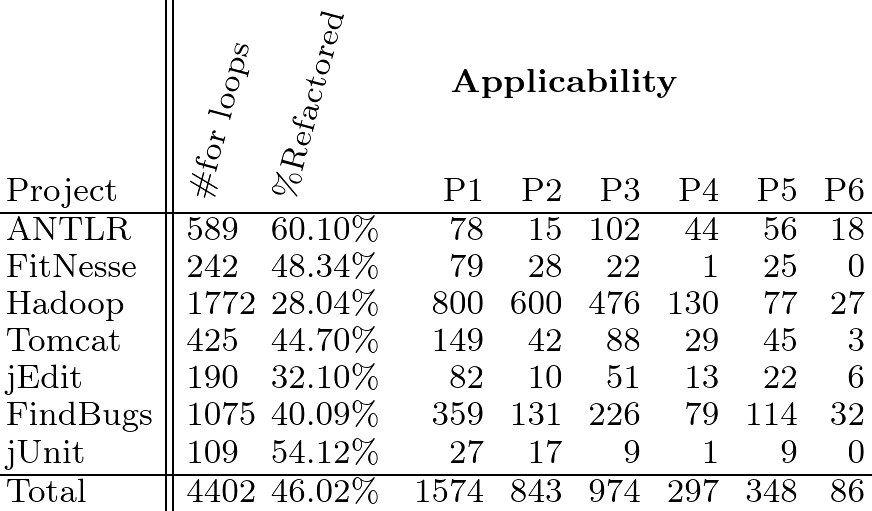
\includegraphics[width=\textwidth,height=.8\textheight,keepaspectratio]{forapp}
\end{column}
\begin{column}{0.2\textwidth}
  P1が高い:配列で拡張for文が多い

  P3が高い:非finalローカル変数を触ってるコード
\end{column}
\end{columns}
\end{frame}

\begin{frame}{ForLoopToFunctionalの価値}
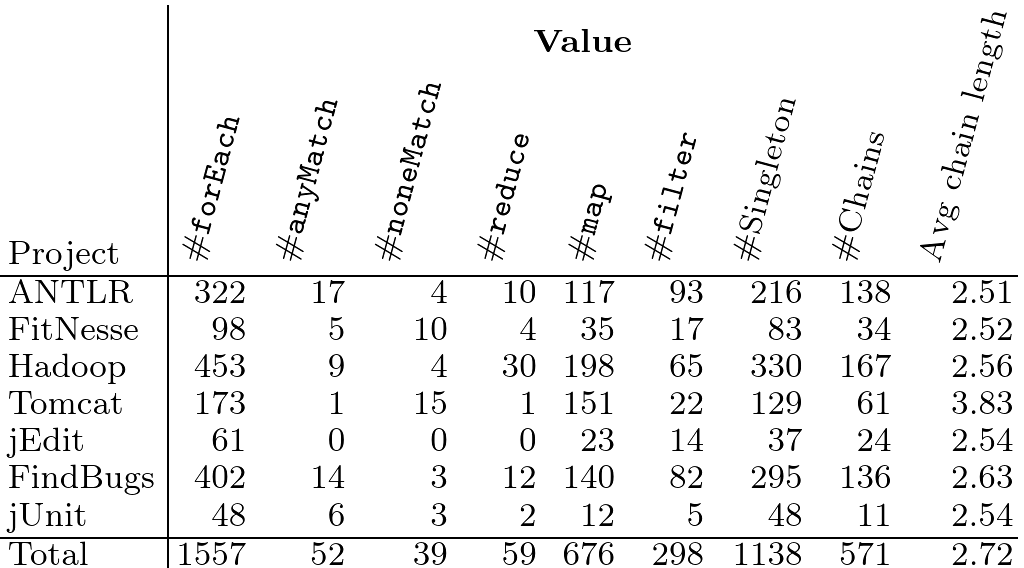
\includegraphics[width=\textwidth,height=.8\textheight,keepaspectratio]{forvalue}
\end{frame}

\begin{frame}{ForLoopToFunctionalの効果と精度}
  \begin{columns}
    \begin{column}{0.4\textwidth}
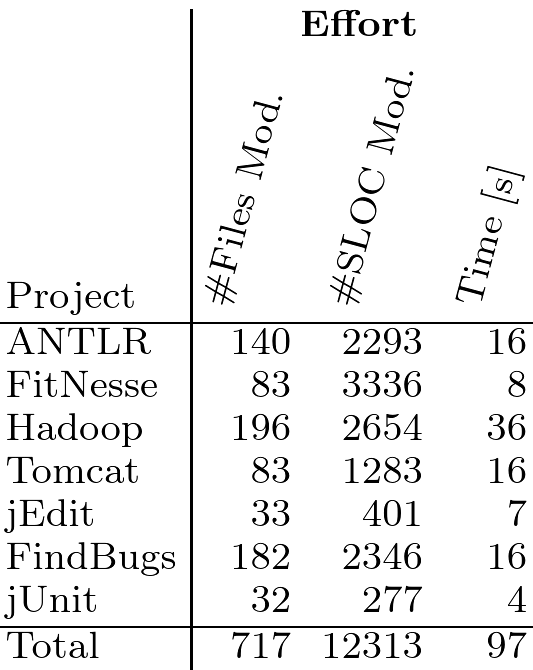
\includegraphics[width=\textwidth,height=.8\textheight,keepaspectratio]{foreffort}
\end{column}
\begin{column}{0.6\textwidth}
  精度に関して
  \begin{block}{precision = 90\%}
  専門家は操作を連鎖する癖がある\\
  意味的には同じコード
  \end{block}

  \begin{block}{recall = 92\%}
  対象外の操作が使える(Stream.min等) \\
  \texttt{reduce}に関するヒューリスティック法が改善の余地がある
  \end{block}
\end{column}
\end{columns}
\end{frame}
%%%%%%%%%%%%%%%%%%%%%%%%%%%%%%%%%%%%%%%%%%%%%%%%%%%%%%%%%%%%%%%%%%%%%%%%
\begin{frame}[fragile]{reduceのヒューリスティック法はうまく行かない例}
ツールの出力
\begin{lstlisting}[morekeywords={map,filter,reduce,forEach,anyMatch,noneMatch}]
List<String> result = new ArrayList<>();
childClassLoaders.entrySet().stream()
  .filter( entry -> isValid(entry))
  .forEach( entry -> {
    ClassLoader cl = entry.getKey();
    if (!((WebappClassLoader)cl).isStart())
      result.add(entry.getValue());
  });
\end{lstlisting}
もっといい案
\begin{lstlisting}[morekeywords={map,filter,reduce,forEach,anyMatch,noneMatch}]
List<String> result = childClassLoaders.entrySet().stream()
  .filter( entry -> isValid(entry) )
  .filter( entry -> !((WebappClassLoader)entry.getKey()).isStart() )
  .map( entry -> Arrays.asList(entry) )
  .reduce(new ArrayList<String>(), List::addAll);
\end{lstlisting}
\end{frame}
%%%%%%%%%%%%%%%%%%%%%%%%%%%%%%%%%%%%%%%%%%%%%%%%%%%%%%%%%%%%%%%%%%%%%%%%
\subsection{妥当性への脅威(Threads to Validity)}
\begin{frame}{妥当性への脅威}{Threads to Validity}
\begin{description}
  \item[構造的妥当性] 開発の作業量を行数やASTのノード数で評価できるか?\\
                      理想的には開発者がツールを使っている様子を観察したいが\ldots
  \item[内部的妥当性] 手作業で作られた正解集合は開発者に違いが生じるか?\\
                      正解集合を作る開発者は全部Javaラムダ式に関する専門家
  \item[外部的妥当性] 実験で得られる結果は他のプロジェクトにも汎用できるか?\\
                      百万を超える行数の性質が違うプロジェクトを9個実験した
  \item[信頼性]       実験の方法やデータが信頼できるか?\\
                      ツールや実験環境は公開した
                      \footnote{\url{http://refactoring.info/tools/LambdaFicator/}}
\end{description}
\end{frame}
%%%%%%%%%%%%%%%%%%%%%%%%%%%%%%%%%%%%%%%%%%%%%%%%%%%%%%%%%%%%%%%%%%%%%%%%
\section{議論と結論}
\subsection{議論(Discussion)}
\begin{frame}{議論}{Discussion}
ラムダ式の引数に型をつけるべきか?
\begin{itemize}
  \item コンパイラーが推測できるから、付けないほう短くて読みやすいが\ldots
  \item 付けるほうが保守性にいい\footfullcite{pankratius2012combining}
  \item プログランマーに選択できる
\end{itemize}
拡張for文の他に、旧式のfor文はどう?
\begin{itemize}
  \item 先行研究に旧式for文を拡張for文に変換する研究があった\footfullcite{java5for}
\end{itemize}
\end{frame}
%%%%%%%%%%%%%%%%%%%%%%%%%%%%%%%%%%%%%%%%%%%%%%%%%%%%%%%%%%%%%%%%%%%%%%%%
\begin{frame}{議論: 自動並列化}{Discussion: Automatic Parallelism}
並列化を自動化しないか?
\begin{itemize}
  \item 先行研究でloop文を並列化のスケーラビリティを議論した\footfullcite{bocchino2009type}
  \item プログランマーに正確性を確かめたうえ、簡単にできる\\
        \texttt{collection.\color{red}{stream}()} $\rightarrow$ \texttt{collection.\color{red}{parallelStream}()}
  \item 先行研究としてdata-race detector\footfullcite{radoi2013practical}もあった、組み合わせて使える
\end{itemize}
\end{frame}
%%%%%%%%%%%%%%%%%%%%%%%%%%%%%%%%%%%%%%%%%%%%%%%%%%%%%%%%%%%%%%%%%%%%%%%%
\subsection{結論(Conclusions)}
\begin{frame}{結論}{Conclusions}
  この研究では2つのリファクタリング手法を提案した
  \begin{itemize}
    \item AnonymousToLambda
    \item ForLoopToFunctional
  \end{itemize}
  それぞれ設計し、NetBeansの一部として実装し、実験した。

  論文は発表時に、Java 8はまだ公開していない
  \begin{itemize}
    \item 初めてJava言語の新機能とそれを補助するツールが一緒にプログランマーに提供
    \item ラムダ式新機能の普及に役立てたらいいなぁ
  \end{itemize}
\end{frame}
%%%%%%%%%%%%%%%%%%%%%%%%%%%%%%%%%%%%%%%%%%%%%%%%%%%%%%%%%%%%%%%%%%%%%%%%
\backupbegin

\begin{frame}

  \center \Huge ありがとうございました
\end{frame}

\backupend
\end{document}
